 1. A stationary tuning fork is in resonance with an air column in a pipe. If the tuning fork is moved with a speed of \(2\text{ m s}^{-1}\) in front of the open end of the pipe and parallel to it, the length of the pipe should be changed for the resonance to occur with the moving tuning fork. If the speed of sound in air is \(320\text{ m s}^{-1}\), the smallest value of the percentage change required in the length of the pipe is _____.

\begin{center}
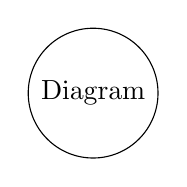
\begin{tikzpicture}
  \node [draw, shape=circle] {Diagram};
\end{tikzpicture}
\end{center}